\documentclass[14pt]{extarticle}
\usepackage[margin=1in]{geometry}
\usepackage{amsmath}
\usepackage{enumitem}
\usepackage{titlesec}
\usepackage{algorithm}
\usepackage{algpseudocode}
\usepackage{hyperref}
\usepackage{caption}
\usepackage{float}
\usepackage{listings}
\usepackage{xcolor}
\usepackage{booktabs}
\usepackage{tikz}
\usepackage{enumitem}
\usepackage{caption}

% Code styling
\lstdefinestyle{python}{
  language=Python,
  basicstyle=\ttfamily\small,
  keywordstyle=\color{blue},
  commentstyle=\color{gray},
  stringstyle=\color{orange},
  showstringspaces=false,
  numbers=left,
  numberstyle=\tiny\color{gray},
  breaklines=true,
  frame=single,
  tabsize=4,
  captionpos=b
}

\lstdefinestyle{cpp}{
  language=C++,
  basicstyle=\ttfamily\small,
  keywordstyle=\color{blue},
  commentstyle=\color{gray},
  stringstyle=\color{orange},
  showstringspaces=false,
  numbers=left,
  numberstyle=\tiny\color{gray},
  breaklines=true,
  frame=single,
  tabsize=4,
  captionpos=b
}

\title{Job Sequencing with Deadline: A Greedy Approach}
\author{Varun Kumar}
\date{\today}

\begin{document}
\maketitle
\newpage
\tableofcontents

\lstlistoflistings
\listofalgorithms
\newpage

\section{Introduction}
The \textbf{Job Sequencing with Deadline} problem involves scheduling jobs to maximize total profit when each job has:
\begin{itemize}
    \item a \textbf{profit} value
    \item a \textbf{deadline}
    \item takes \textbf{one unit of time}
\end{itemize}

\textbf{Goal:} Maximize total profit by completing jobs within their deadline, assuming only one job can be scheduled at a time.

\section{Problem Statement}
Given $n$ jobs, each with:
\begin{itemize}
    \item Job ID
    \item Deadline (integer)
    \item Profit
\end{itemize}
Schedule the jobs to maximize profit such that no two jobs overlap and each job is done before or on its deadline.

\section{Approach: Greedy Algorithm}
\begin{itemize}
    \item Sort all jobs in descending order of profit.
    \item Create a result array to store job sequence and track free slots.
    \item For each job, find the latest available slot before its deadline.
    \item If a slot is found, schedule it.
\end{itemize}

%%%%%%%%%%%%% An Example %%%%%%%%%%%%%
\subsection{Problem Statement}
Given 5 jobs with deadlines and profits:

\begin{center}
\begin{tabular}{|c|c|c|}
\hline
\textbf{Job ID} & \textbf{Deadline} & \textbf{Profit} \\
\hline
J1 & 2 & 60 \\
J2 & 1 & 100 \\
J3 & 3 & 20 \\
J4 & 2 & 40 \\
J5 & 1 & 20 \\
\hline
\end{tabular}
\end{center}

\textbf{Goal:} Schedule jobs to maximize total profit. Each job takes 1 unit of time and must be finished before or on its deadline.

\subsection{Step 1: Sort Jobs by Profit (Descending)}

\begin{center}
\begin{tabular}{|c|c|c|}
\hline
\textbf{Job ID} & \textbf{Deadline} & \textbf{Profit} \\
\hline
J2 & 1 & 100 \\
J1 & 2 & 60 \\
J4 & 2 & 40 \\
J3 & 3 & 20 \\
J5 & 1 & 20 \\
\hline
\end{tabular}
\end{center}

\subsection{Step 2: Schedule Jobs in Greedy Manner}

We’ll use a time slot array. The maximum deadline is 3, so we have 3 time slots: Slot 1, Slot 2, Slot 3.

\begin{enumerate}[label=\textbf{Job \arabic*:}]
    \item \textbf{J2:} Deadline 1 → Slot 1 is free → Schedule J2 at Slot 1
    \item \textbf{J1:} Deadline 2 → Slot 2 is free → Schedule J1 at Slot 2
    \item \textbf{J4:} Deadline 2 → Slot 2 is full → Check Slot 1 (already taken) → Can't schedule
    \item \textbf{J3:} Deadline 3 → Slot 3 is free → Schedule J3 at Slot 3
    \item \textbf{J5:} Deadline 1 → Slot 1 is full → Can't schedule
\end{enumerate}

\subsection{Step 3: Final Scheduled Jobs}

\begin{center}
\begin{tabular}{|c|c|}
\hline
\textbf{Time Slot} & \textbf{Job Scheduled} \\
\hline
Slot 1 & J2 \\
Slot 2 & J1 \\
Slot 3 & J3 \\
\hline
\end{tabular}
\end{center}

\textbf{Total Profit} = 100 (J2) + 60 (J1) + 20 (J3) = \textbf{180}

\subsection{Step 4: Timeline Visualization}

\begin{center}
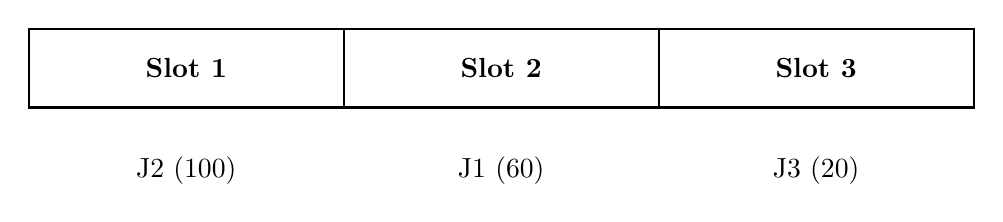
\begin{tikzpicture}
% Draw time slots
\foreach \x in {0,1,2} {
    \draw[thick] (\x*4,0) rectangle ++(4,1);
    \node at (\x*4 + 2, 0.5) {\textbf{Slot \number\numexpr\x+1}};
}

% Draw job labels
\node at (2, -0.8) {J2 (100)};
\node at (6, -0.8) {J1 (60)};
\node at (10, -0.8) {J3 (20)};
\end{tikzpicture}
\end{center}

\subsection{Conclusion}
Using the greedy strategy:
\begin{itemize}
    \item We prioritized jobs with the highest profit.
    \item Placed each job in the latest available slot before its deadline.
    \item Achieved maximum profit of \textbf{180}.
\end{itemize}

This is an efficient solution with time complexity:
\[
O(n \log n + n \cdot d)
\]
where $d$ is the maximum deadline.

\newpage
%%%%%%%%%% Logic and Implementation %%%%%%%%%%
\section{Theoretical Logic Behind Job Sequencing with Deadline Code Implementation}

The Job Sequencing with Deadline problem is solved using a \textbf{greedy algorithm} aimed at maximizing total profit. Each job has:
\begin{itemize}
    \item A \textbf{deadline} (latest time by which it must be scheduled)
    \item A \textbf{profit} (earned if scheduled before or on the deadline)
\end{itemize}

\subsection*{Approach Overview}

\begin{enumerate}
    \item Sort all jobs in \textbf{descending order of profit}.
    \item Initialize a time slot array of size equal to the \textbf{maximum deadline}.
    \item Iterate over each job in sorted order:
    \begin{itemize}
        \item Try to place the job in the \textbf{latest available slot} on or before its deadline.
        \item If such a slot exists, assign the job and accumulate the profit.
    \end{itemize}
    \item Continue until all jobs are considered.
\end{enumerate}

\subsection*{Why Greedy Works}

The problem satisfies:
\begin{itemize}
    \item \textbf{Greedy choice property:} Locally best choice (most profitable job first) leads to global optimum.
    \item \textbf{Optimal substructure:} Scheduling earlier jobs doesn't prevent optimal scheduling of remaining jobs.
\end{itemize}

\subsection*{Time and Space Complexity}

\begin{itemize}
    \item \textbf{Sorting:} $O(n \log n)$
    \item \textbf{Scheduling:} $O(n \cdot d)$ where $d$ is the max deadline (or $O(n)$ with Disjoint Set Union)
    \item \textbf{Space:} $O(d)$ for the slot array
\end{itemize}

\subsection*{Slot Allocation Strategy}

For each job with deadline $d_i$, we look for a free slot from $d_i$ to $1$. The goal is to place the job as \textbf{late as possible} before its deadline to leave earlier slots open for tighter-deadline jobs.

\textbf{Example:}  
If Job A has deadline 3, we try: Slot 3 $\rightarrow$ Slot 2 $\rightarrow$ Slot 1.  
This backward check ensures maximum slot availability for other jobs.

\subsection*{Final Result}

The algorithm outputs:
\begin{itemize}
    \item A list of scheduled jobs
    \item Maximum total profit earned
\end{itemize}
This solution is efficient and optimal for single-unit jobs under hard deadlines.

\subsection{Pseudocode}
\begin{algorithm}[H]
\caption{Job Sequencing with Deadline}
\begin{algorithmic}[1]
\Procedure{jobSequencing}{$jobs$}
    \State Sort jobs by descending profit
    \State $result \gets$ array of size max\_deadline
    \State $slot \gets$ array of size max\_deadline initialized as False
    \For{each job in jobs}
        \For{$j = \min(job.deadline, n) - 1$ to $0$}
            \If{slot[j] == False}
                \State result[j] $\gets$ job
                \State slot[j] $\gets$ True
                \State \textbf{break}
            \EndIf
        \EndFor
    \EndFor
    \State \Return scheduled jobs from result
\EndProcedure
\end{algorithmic}
\end{algorithm}

\newpage
\subsection{Python Implementation}
\begin{lstlisting}[style=python, caption={Job Sequencing with Deadline in Python}]
class Job:
    def __init__(self, id, deadline, profit):
        self.id = id
        self.deadline = deadline
        self.profit = profit

def job_sequencing(jobs):
    jobs.sort(key=lambda x: x.profit, reverse=True)
    max_deadline = max(job.deadline for job in jobs)
    result = [None] * max_deadline
    slot = [False] * max_deadline

    for job in jobs:
        for j in range(min(max_deadline, job.deadline)-1, -1, -1):
            if not slot[j]:
                result[j] = job.id
                slot[j] = True
                break

    return [job_id for job_id in result if job_id]
\end{lstlisting}

\newpage
\subsection{C++ Implementation}
\begin{lstlisting}[style=cpp, caption={Job Sequencing with Deadline in C++}]
#include <iostream>
#include <vector>
#include <algorithm>
using namespace std;
struct Job {
    char id;
    int deadline, profit;
};
bool cmp(Job a, Job b) {
    return a.profit > b.profit;
}
vector<char> jobSequencing(vector<Job> &jobs) {
    sort(jobs.begin(), jobs.end(), cmp);
    int max_deadline = 0;
    for (Job &job : jobs) max_deadline = max(max_deadline, job.deadline);
    vector<char> result(max_deadline, '\0');
    vector<bool> slot(max_deadline, false);
    for (Job &job : jobs) {
        for (int j = min(job.deadline, max_deadline) - 1; j >= 0; --j) {
            if (!slot[j]) {
                result[j] = job.id;
                slot[j] = true;
                break;
            }
        }
    }
    vector<char> scheduled;
    for (char c : result) {
        if (c != '\0') scheduled.push_back(c);
    }
    return scheduled;
}
\end{lstlisting}

\newpage
\section{Key Points to Remember}
\begin{enumerate}
    \item Greedy approach: always pick highest profit job first.
    \item Sorting based on profit is crucial.
    \item Use a time-slot array to track free positions.
    \item Try to place each job in the latest available slot.
    \item Each job takes 1 unit of time.
\end{enumerate}

\section{Time and Space Complexity}
\begin{itemize}
    \item \textbf{Time:} $O(n \log n + n \cdot d)$ where $d$ is max deadline
    \item \textbf{Space:} $O(d)$ for time slot tracking
\end{itemize}

\section{Real-World Applications}
\begin{itemize}
    \item \textbf{CPU Job Scheduling:} Maximize efficiency and throughput
    \item \textbf{Project Deadlines:} Pick best paying contracts under time constraint
    \item \textbf{Cloud Computing:} Efficient resource utilization for tasks
    \item \textbf{Freelancing:} Prioritize clients with highest returns before due dates
\end{itemize}

\section{Conclusion}
Job Sequencing with Deadline is a fundamental greedy algorithm that models real-world scheduling and optimization problems. It ensures profit maximization while adhering to time constraints — a key strategy in resource management and systems design.

\end{document}
